% Arbres généalogiques (actes d'état civil, faire-part, fichier INSEE des décès, études familiales
% de Pierre Combes). Personnes vivantes : nom et lien seulement.
\tikzset{
  LJp/.style={draw=black!70, line width=0.35pt, rounded corners=1pt, fill=white, inner sep=1.4pt,
              align=center, font=\fontsize{6.3pt}{7.4pt}\selectfont, text width=#1,
              execute at begin node={\hyphenpenalty=10000\relax\exhyphenpenalty=10000\relax}},
  LJp/.default=21mm,
  LJh/.style={LJp=#1, draw=black, line width=0.9pt, double, double distance=0.5pt},
  LJh/.default=27mm,
  LJl/.style={draw=black!65, line width=0.4pt},
  LJm/.style={font=\fontsize{5.6pt}{6.4pt}\selectfont\itshape, text=black!75, fill=white, inner sep=0.6pt},
}

\begin{figure}[p]
\centering
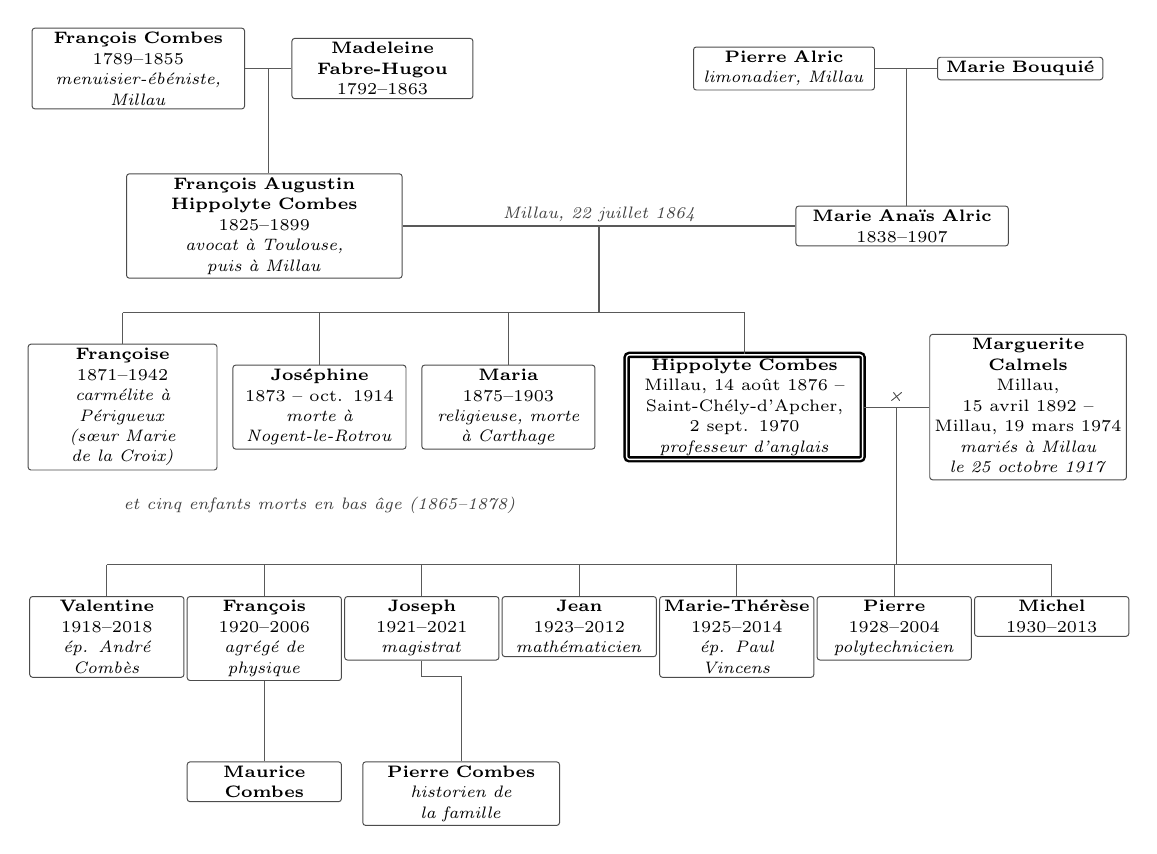
\begin{tikzpicture}[x=1mm,y=1mm]
  % --- grands-parents ---
  \node[LJp=26mm] (fc) at (14,0) {\textbf{François Combes}\\1789–1855\\\textit{menuisier-ébéniste, Millau}};
  \node[LJp=22mm] (mf) at (45,0) {\textbf{Madeleine Fabre-Hugou}\\1792–1863};
  \node[LJp=22mm] (pa) at (96,0) {\textbf{Pierre Alric}\\\textit{limonadier, Millau}};
  \node[LJp=20mm] (mb) at (126,0) {\textbf{Marie Bouquié}};
  \draw[LJl] (fc) -- (mf) coordinate[midway] (u1);
  \draw[LJl] (pa) -- (mb) coordinate[midway] (u2);
  % --- parents ---
  \node[LJp=34mm] (hp) at (30,-20) {\textbf{François Augustin Hippolyte Combes}\\1825–1899\\\textit{avocat à Toulouse, puis à Millau}};
  \node[LJp=26mm] (ma) at (111,-20) {\textbf{Marie Anaïs Alric}\\1838–1907};
  \draw[LJl] (u1) -- (u1 |- hp.north);
  \draw[LJl] (u2) -- (u2 |- ma.north);
  \draw[LJl] (hp) -- (ma) coordinate[pos=0.5] (u3) node[LJm, midway, above=0.3mm] {Millau, 22~juillet 1864};
  % --- fratrie ---
  \node[LJp=23mm] (fr) at (12,-43) {\textbf{Françoise}\\1871–1942\\\textit{carmélite à Périgueux}\\\textit{(sœur Marie de la Croix)}};
  \node[LJp=21mm] (jo) at (37,-43) {\textbf{Joséphine}\\1873 – oct. 1914\\\textit{morte à Nogent-le-Rotrou}};
  \node[LJp=21mm] (mr) at (61,-43) {\textbf{Maria}\\1875–1903\\\textit{religieuse, morte à Carthage}};
  \node[LJh=29mm] (hc) at (91,-43) {\textbf{Hippolyte Combes}\\Millau, 14~août 1876 –\\Saint-Chély-d'Apcher, 2~sept. 1970\\\textit{professeur d'anglais}};
  \node[LJp=24mm] (mc) at (127,-43) {\textbf{Marguerite Calmels}\\Millau, 15~avril 1892 –\\Millau, 19~mars 1974\\\textit{mariés à Millau le 25~octobre 1917}};
  \coordinate (b1) at (u3 |- 0,-31);
  \draw[LJl] (u3) -- (b1);
  \draw[LJl] (fr.north |- b1) -- (hc.north |- b1);
  \foreach \n in {fr,jo,mr,hc} \draw[LJl] (\n.north |- b1) -- (\n.north);
  \node[LJm] at (37,-55.5) {et cinq enfants morts en bas âge (1865--1878)};
  \draw[LJl] (hc) -- (mc) coordinate[midway] (u4) node[LJm, midway, above=0.2mm] {×};
  % --- enfants ---
  \foreach \x/\n/\t in {10/va/{\textbf{Valentine}\\1918–2018\\\textit{ép. André Combès}},
                         30/fo/{\textbf{François}\\1920–2006\\\textit{agrégé de physique}},
                         50/js/{\textbf{Joseph}\\1921–2021\\\textit{magistrat}},
                         70/je/{\textbf{Jean}\\1923–2012\\\textit{mathématicien}},
                         90/mt/{\textbf{Marie-Thérèse}\\1925–2014\\\textit{ép. Paul Vincens}},
                         110/pi/{\textbf{Pierre}\\1928–2004\\\textit{polytechnicien}},
                         130/mi/{\textbf{Michel}\\1930–2013}}
    \node[LJp=18.6mm, anchor=north] (\n) at (\x,-67) {\t};
  \coordinate (b2) at (u4 |- 0,-63);
  \draw[LJl] (u4) -- (b2);
  \draw[LJl] (va.north |- b2) -- (mi.north |- b2);
  \foreach \n in {va,fo,js,je,mt,pi,mi} \draw[LJl] (\n.north |- b2) -- (\n.north);
  % --- petits-fils liés au carnet ---
  \node[LJp=18.6mm, anchor=north] (mau) at (30,-88) {\textbf{Maurice Combes}};
  \node[LJp=24mm, anchor=north] (pie) at (55,-88) {\textbf{Pierre Combes}\\\textit{historien de la famille}};
  \draw[LJl] (fo.south) -- (mau.north);
  \draw[LJl] (js.south) -- ++(0,-2) -| (pie.north);
\end{tikzpicture}
\caption{La famille d'Hippolyte Combes : ascendance, fratrie, descendance.}
\label{arbre-combes}

\vspace{6mm}

\begin{tikzpicture}[x=1mm,y=1mm]
  % --- grands-parents de Marguerite ---
  \node[LJp=30mm] (jc) at (17,0) {\textbf{Joseph Hippolyte Calmels}\\né en 1814\\\textit{docteur en médecine, Millau}};
  \node[LJp=22mm] (jb) at (48,0) {\textbf{Julie Magdelaine Boyer}\\née en 1824};
  \node[LJp=24mm] (gc) at (94,0) {\textbf{Guillaume Cartairade}};
  \node[LJp=22mm] (en) at (126,0) {\textbf{Émilie Noel}\\† 1889};
  \draw[LJl] (jc) -- (jb) coordinate[midway] (v1);
  \draw[LJl] (gc) -- (en) coordinate[midway] (v2);
  % --- génération des parents ---
  \node[LJp=24mm] (ec) at (13,-21) {\textbf{Élisabeth Calmels}\\× Émile Crouzet\\\textit{(† 1926)}};
  \node[LJp=14mm] (ac) at (35,-21) {\textbf{Anne Calmels}};
  \node[LJp=24mm] (gab) at (58,-21) {\textbf{Gabriel Calmels}\\1852–1921\\\textit{médecin à Millau}};
  \node[LJp=24mm] (vc) at (88,-21) {\textbf{Valentine Cartairade}\\1858–1943};
  \node[LJp=22mm] (tc) at (114,-21) {\textbf{Thérèse Cartairade}\\× Charles Layral\\\textit{notaire à Millau}};
  \node[LJp=12mm] (ar) at (133.5,-21) {M\textsuperscript{me} Ernest Arnal};
  \coordinate (c1) at (v1 |- 0,-11);
  \draw[LJl] (v1) -- (c1);
  \draw[LJl] (ec.north |- c1) -- (gab.north |- c1);
  \foreach \n in {ec,ac,gab} \draw[LJl] (\n.north |- c1) -- (\n.north);
  \coordinate (c2) at (v2 |- 0,-11);
  \draw[LJl] (v2) -- (c2);
  \draw[LJl] (vc.north |- c2) -- (ar.north |- c2);
  \foreach \n in {vc,tc,ar} \draw[LJl] (\n.north |- c2) -- (\n.north);
  \draw[LJl] (gab) -- (vc) coordinate[midway] (v3);
  % --- génération de Marguerite ---
  \node[LJp=20mm, anchor=north] (jcr) at (13,-37) {\textbf{abbé Jean Crouzet}\\† 1932};
  \node[LJp=22mm, anchor=north] (mad) at (39,-37) {\textbf{Madeleine}\\\textit{ép. le D\textsuperscript{r} Fernand Vincens}};
  \node[LJp=17mm, anchor=north] (pie) at (60,-37) {\textbf{Pierre}\\1884–1924\\\textit{médecin}};
  \node[LJp=19mm, anchor=north] (mim) at (79.5,-37) {\textbf{Anne-Marie}\\«~Mimi~»\\1888–1975\\\textit{ép. Joseph Delcamps}};
  \node[LJh=22mm, anchor=north] (mg) at (100.5,-37) {\textbf{Marguerite}\\1892–1974\\\textit{ép. Hippolyte Combes}};
  \node[LJp=15mm, anchor=north] (lay) at (128,-37) {\textbf{Louis} et \textbf{Jean Layral}};
  \draw[LJl] (ec.south) -- (jcr.north);
  \coordinate (c3) at (v3 |- 0,-33);
  \draw[LJl] (v3) -- (c3);
  \draw[LJl] (mad.north |- c3) -- (mg.north |- c3);
  \foreach \n in {mad,pie,mim,mg} \draw[LJl] (\n.north |- c3) -- (\n.north);
  \draw[LJl] (tc.south) -- ++(0,-2) -| (lay.north);
  \node[LJp=28mm, anchor=north] (vin) at (39,-55) {\textbf{Germaine}, \textbf{Robert}, \textbf{Paul},\\\textbf{D\textsuperscript{r} Gabriel («~Gaby~»)}\\\textit{et leurs frères et sœurs Vincens}};
  \draw[LJl] (mad.south) -- (vin.north);
  \node[LJm, anchor=north west, text width=72mm, align=left] at (66,-56) {Branche Fabry–Faure : Eugénie-Joséphine Calmels, sœur de Joseph Hippolyte, ép. Charles Fabry, notaire à Millau. Sa petite-fille Marguerite Barnerot, M\textsuperscript{me} Camille Faure, vivait à Neuilly avec ses enfants Henri († 1918), André, Germaine et Marcel. Branches Combes, Calmels et Vincens d'après les recherches de Pierre Combes et de Nicole Vincens, fille du D\textsuperscript{r} Gabriel («~Gaby~») Vincens.};
\end{tikzpicture}
\caption{La famille de Marguerite Calmels : Calmels, Cartairade et alliés.}
\label{arbre-calmels}
\end{figure}
